\section{QUY TẮC CỘNG VÀ QUY TẮC NHÂN}
\subsection{LÝ THUYẾT CẦN NHỚ}

\subsubsection{Quy tắc cộng}
\noindent Giả sử một công việc có thể được thực hiện theo phương án $A$ hoặc phương án $B$. Phương án $A$ có $m$ cách thực hiện, phương án $B$ có $n$ cách thực hiện không trùng với bất kỳ cách nào của phương án $A$. Khi đó, công việc có thể thực hiện theo $m+n$ cách.
\subsubsection{Quy tắc nhân}
\noindent Giả sử một công việc được chia thành hai công đoạn. Công đoạn thứ nhất có $m$ cách thực hiện và ứng với mỗi cách thực hiện đó có $n$ cách thực hiện công đoạn thứ hai. Khi đó, công việc có thể thực hiện theo $m \cdot n$ cách.

\subsection{PHÂN LOẠI VÀ PHƯƠNG PHÁP GIẢI TOÁN}
\begin{dang}{Đếm bằng quy tắc cộng}
\end{dang}

\begin{vd}%[0D8N1-1]%[Dự án đề cương 3 khối NH24-25-Dot 1-Thy Nguyen Vo Diem]
	Lớp $10A$ có $36$ học sinh, lớp $10B$ có $40$ học sinh. Có bao nhiêu cách cử một học sinh của lớp $10A$ hoặc của lớp $10B$ tham gia một công việc tình nguyện sắp diễn ra?
	\loigiai{
		Công việc cử một học sinh có hai phương án thực hiện.\\
		\textit{Phương án 1:} Cử một học sinh của lớp $10A$, có $36$ cách thực hiện.\\
		\textit{Phương án 2:} Cử một học sinh của lớp $10B$, có $40$ cách thực hiện.\\
		Ta thấy mỗi cách thực hiện của phương án này không trùng với bất kỳ cách nào của phương án kia. Do đó, theo quy tắc cộng, có $36+40=76$ cách cử một học sinh trong hai lớp tham gia công việc tình nguyện.}
\end{vd}
\begin{vd}%[0D8N1-1]%[Dự án đề cương 3 khối NH24-25-Dot 1-Thy Nguyen Vo Diem]
	Mỗi ngày có $6$ chuyến xe khách, $3$ chuyến tàu hỏa và $4$ chuyến máy bay từ thành phố $A$ đến thành phố $B$. Mỗi ngày có bao nhiêu cách chọn chuyến để di chuyển từ thành phố $A$ đến thành phố $B$ bằng một trong ba loại phương tiện trên?
	\loigiai{
		Việc di chuyển từ $A$ đến $B$ có ba phương án thực hiện.\\
		\textit{Phương án 1:} Di chuyển bằng xe khách, có $6$ cách.\\
		\textit{Phương án 2:} Di chuyển bằng tàu hỏa, có $3$ cách.\\
		\textit{Phương án 3:} Di chuyển bằng máy bay, có $4$ cách.\\
		Áp dụng quy tắc cộng, ta có số cách chọn để di chuyển từ $A$ đến $B$ là $6+3+4=13$ (cách).
	}
\end{vd}
\begin{vd}%[0D8N1-1]%[Dự án đề cương 3 khối NH24-25-Dot 1-Thy Nguyen Vo Diem]
	Hà có $5$ cuốn sách khoa học, $4$ cuốn tiểu thuyết và $3$ cuốn truyện tranh (các sách khác nhau từng đôi một). Hà đồng ý cho Nam mượn một cuốn sách trong số đó để đọc. Nam có bao nhiêu cách chọn một cuốn sách để mượn?
	\loigiai{
		Công việc mượn sách có $3$ phương án để thực hiện.\\
		\textit{Phương án 1:} Mượn sách khoa học, có $5$ cách thực hiện.\\
		\textit{Phương án 2:} Mượn sách tiểu thuyết, có $4$ cách thực hiện.\\
		\textit{Phương án 3:} Mượn truyện tranh, có $3$ cách thực hiện.\\ 	
		Áp dụng quy tắc cộng, ta có $5+4+3=12$ (cách).
	}
\end{vd}	

\begin{dang}{Đếm bằng quy tắc nhân}
	
\end{dang}

\begin{vd}%[0D8H1-2]%[Dự án đề cương 3 khối NH24-25-Dot 1-Thy Nguyen Vo Diem]
	Có ba thị trấn $A$, $B$, $C$.  Có $5$ con đường để đi từ $A$ đến $B$, có $3$ con đường  để đi từ $B$ đến $C$. Có bao nhiêu cách chọn một con đường để đi từ $A$, qua $B$ rồi đến $C$?
	\loigiai{
		Việc đi từ $A$, qua $B$ rồi đến $C$ gồm hai công đoạn:\\
		\textit{Công đoạn thứ nhất:} Đi từ $A$ đến $B$, có $5$ con đường đi.\\
		\textit{Công đoạn thứ hai:} Ứng với mỗi cách chọn đường đi từ $A$ đến $B$, có $3$ cách chọn đường đi từ $B$ đến $C$.\\
		Theo quy tắc nhân, có $5 \cdot 3 = 15$ cách chọn để đi từ $A$, qua $B$ rồi đến $C$.	
	}
\end{vd}	
\begin{vd}%[0D8N1-2]%[Dự án đề cương 3 khối NH24-25-Dot 1-Thy Nguyen Vo Diem]
	Nam muốn tô màu cho $1$ hình vuông hoặc $1$ hình tròn, biết rằng chỉ có thể tô màu xanh, màu đỏ hoặc màu vàng cho hình vuông, và chỉ có thể tô màu hồng hoặc màu tím cho hình tròn. Hỏi Nam có bao nhiêu cách tô màu cho $2$ hình?
	\choice
	{$2$ cách}
	{$3$ cách}
	{$5$ cách}
	{\True $6$ cách}
	\loigiai{
		Tô màu cho hình vuông: có $2$ cách.\\
		Tô màu cho hình tròn: có $3$ cách.\\
		Vậy có $2\cdot 3=6$ cách tô màu cho $2$ hình.
	}
\end{vd}
\begin{dang}{Đếm bằng quy tắc cộng kết hợp quy tắc nhân}
\end{dang}

\begin{vd}%[0D8H1-5]%[Dự án đề cương 3 khối NH24-25-Dot 1-Thy Nguyen Vo Diem]
	Từ năm chữ số $0$, $1$, $2$, $3$, $4$ có thể lập được bao nhiêu
	\begin{enumerate}
		\item số tự nhiên có ba chữ số đôi một khác nhau?
		\item số tự nhiên chẵn có ba chữ số đôi một khác nhau?
	\end{enumerate}
	\loigiai{
		Kí hiệu số cần lập là $\overline{abc}$, với $a$, $b$, $c$ là ba chữ số đôi một khác nhau từ các số đã cho.
		\begin{enumerate}
			\item Có $4$ cách lựa chọn chữ số $a$ từ bốn chữ số khác $0$ đã cho.\\
			Ứng với mỗi cách chọn đó, có $4$ cách chọn chữ số $b$ từ bốn chữ số còn lại.\\
			Ứng với mỗi cách chọn đó, có $3$ cách chọn chữ số $c$ từ ba chữ số còn lại.\\
			Từ đó, áp dụng quy tắc nhân, có $4 \cdot 4 \cdot 3 = 48$ số tự nhiên có ba chữ số đôi một khác nhau được lập từ các số đã cho.
			\item Để số $\overline{abc}$ là số chẵn, chữ số $c$ phải là số chẵn. Ta xét hai trường hợp sau đây.
			\begin{itemize}
				\item \textit{Trường hợp 1:} $c=0$. Khi đó, có $4$ cách chọn chữ số $a$ từ bốn chữ số còn lại, và ứng với mỗi cách chọn đó, có $3$ cách chọn chữ số $b$ từ ba số còn lại. Do đó, theo quy tắc nhân, trường hợp này có $4 \cdot 3 = 12$ số thỏa mãn yêu cầu.
				\item \textit{Trường hợp 2:} $c=2$ hoặc $c=4$. Khi đó, có hai cách chọn chữ số $c$ từ hai số $2$ hoặc $4$. Ứng với mỗi cách chọn đó, có $3$ cách chọn chữ số $a$ từ ba số khác $0$ còn lại, và ứng với mỗi cách chọn đó, có $3$ cách chọn chữ số $b$ từ các số còn lại. Do đó, theo quy tắc nhân, trường hợp này có $2 \cdot 3 \cdot 3 = 18$ số thỏa yêu cầu.
			\end{itemize}
			Trong hai trường hợp trên, mỗi số được lập theo trường hợp này đều khác với các số lập được của trường hợp kia.\\
			Theo quy tắc cộng, có $12+18=30$ số tự nhiên chẵn có ba chữ số đôi một khác nhau lập từ các số đã cho.
		\end{enumerate}
	}
\end{vd}

\begin{vd}%[0D8H1-5]%[Dự án đề cương 3 khối NH24-25-Dot 1-Thy Nguyen Vo Diem]
	Từ các chữ số $0$, $1$, $2$, $3$, $4$, $5$ có thể lập được bao nhiêu số tự nhiên gồm bốn chữ số phân biệt và chia hết cho $5$?
	\loigiai{
		Gọi số tự nhiên cần tìm là $\overline{abcd}$.\\
		\textbf{Trường hợp 1:} $d=0$, có $1$ cách chọn $d$.\\
		Chọn $a$ khác $0$: có $5$ cách. Mỗi chữ số $b$, $c$ lần lượt có $4$, $3$ cách chọn.\\
		Vậy số các số tự nhiên trong trường hợp này là $1 \cdot 5 \cdot 4 \cdot 3=60$ (số).\\
		\textbf{Trường hợp 2:} $d=5$, có $1$ cách chọn $d$.\\
		Chọn $a$ khác $d$ và khác $0$: có $4$ cách. Mỗi chữ số $b$, $c$ lần lượt có $4$, $3$ cách chọn.\\
		Vậy số các số tự nhiên trong trường hợp này là $1 \cdot 4 \cdot 3=48$ (số).\\
		Số các số tự nhiên thỏa mãn đề bài: $60+48=108$ (số).
	}
\end{vd}
\begin{dang}{Đếm bằng sơ đồ hình cây}
\end{dang}

\begin{vd}%[0D8H1-6]%[Dự án đề cương 3 khối NH24-25-Dot 1-Thy Nguyen Vo Diem]
	Một đồng xu có hai mặt sấp và ngửa (ký hiệu $S$ và $N$). Tung đồng xu ba lần liên tiếp và ghi lại kết quả có thể xảy ra, theo hai cách sau đây:
	\begin{enumerate}
		\item Vẽ sơ đồ cây.
		\item Sử dụng quy tắc nhân.
	\end{enumerate}
	\loigiai{
		\begin{enumerate}
			\item Vẽ sơ đồ cây.
			\begin{center}
				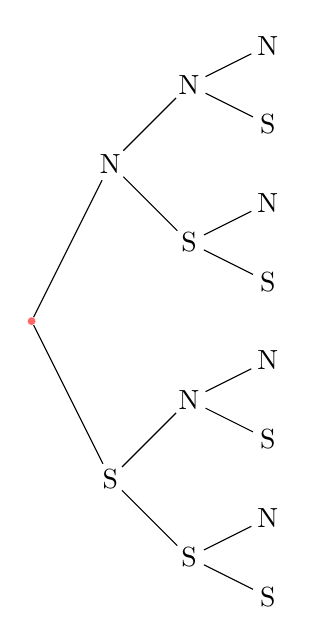
\begin{tikzpicture}
					[level distance=10mm,
					every node/.style={fill=red!60,circle,inner sep=1pt},
					level 1/.style={sibling distance=40mm,nodes={fill=white!30}},
					level 2/.style={sibling distance=20mm},
					level 3/.style={sibling distance=10mm}, rotate = 90]
					\node {}
					child {node {S}
						child {node {S}
							child {node {S}}
							child {node {N}}
						}
						child {node {N}
							child {node {S}}
							child {node {N}}
						}
					}
					child {node {N}
						child {node {S}
							child {node {S}}
							child {node {N}}
						}
						child {node {N}
							child {node {S}}
							child {node {N}}
						}
					}
					;
				\end{tikzpicture}
			\end{center}
			\item Có thể coi việc tung đồng xu ba lần liên tiếp là một công việc gồm ba công đoạn, mỗi công đoạn tương ứng với một lần tung đồng xu. Mỗi lần tung đồng xu có hai kết quả là $S$ hoặc $N$. Do đó, theo quy tắc nhân, số kết quả của việc tung đồng xu ba lần liên tiếp là
			$2 \cdot 2 \cdot 2 = 8$ (kết quả).
		\end{enumerate}
	}
\end{vd}

\begin{vd}%[0D8H1-6]%[Dự án đề cương 3 khối NH24-25-Dot 1-Thy Nguyen Vo Diem]
	Tung đồng thời một đồng xu và một con xúc xắc, nhận được kết quả là mặt xuất hiện trên đồng xu (sấp hay ngửa) và số chấm xuất hiện trên con xúc xắc.
	\begin{enumerate}
		\item Tính số kết quả có thể xảy ra.
		\item Vẽ sơ đồ cây và liệt kê tất cả các kết quả đó.
	\end{enumerate}	
	\loigiai{
		\begin{enumerate}
			\item 
			Công việc gồm hai bước:\\
			\textit{Bước 1:} Tung đồng xu, có $2$ kết quả xảy ra.\\
			\textit{Bước 2:} Tung xúc xắc, có $6$ kết quả xảy ra.\\
			Áp dụng quy tắc nhân, có $2 \cdot 6 =12$ kết quả xảy ra.
			\item Vẽ sơ đồ cây và liệt kê tất cả các kết quả đó.
			\begin{center}
				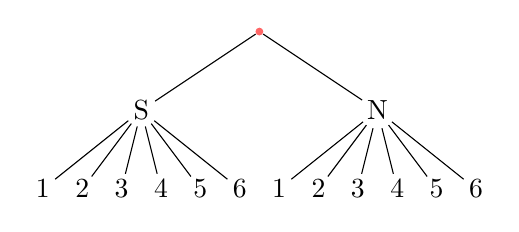
\begin{tikzpicture}
					[level distance=10mm,
					every node/.style={fill=red!60,circle,inner sep=1pt},
					level 1/.style={sibling distance=30mm,nodes={fill=white!30}},
					level 2/.style={sibling distance=5mm},]
					\node {}
					child {node {S}
						child {node {1}}
						child {node {2}}
						child {node {3}}
						child {node {4}}
						child {node {5}}
						child {node {6}}
					}
					child {node {N}
						child {node {1}}
						child {node {2}}
						child {node {3}}
						child {node {4}}
						child {node {5}}
						child {node {6}}
					}
					;
				\end{tikzpicture}
			\end{center}
		\end{enumerate}
	}
\end{vd}

%-----------------------------------------------------------------------------
\subsection{Bài tập rèn luyện}
\ind{PHẦN I.} \inden{Câu trắc nghiệm nhiều phương án lựa chọn. Mỗi câu hỏi học sinh chỉ chọn một phương án.}\\
\setcounter{ex}{0}
\Opensolutionfile{ans}[ans/0D8-Bai1-TN]

\begin{ex}%[0D8N1-1]%[Dự án đề cương 3 khối NH24-25-Dot 1-Thy Nguyen Vo Diem]
	[\textit{Trích đề thi GKII - THPT Chuyên Vị Thanh - Hậu Giang - Năm học 2024-2025}]
	Một trong một cửa hàng bán kem có $6$ loại kem que và $3$ loại kem ốc quế. Có bao nhiêu cách chọn mua một loại kem que hoặc kem ốc quế ở cửa hàng này?
	\choice
	{$6$}
	{$3$}
	{$18$}
	{\True $9$} 
	\loigiai{
		Áp dụng quy tắc cộng, số cách chọn là $6 + 3 = 9$ (cách).
	}
\end{ex}

\begin{ex}%[0D8N1-1]%[Dự án đề cương 3 khối NH24-25-Dot 1-Thy Nguyen Vo Diem]
	[\textit{Trích đề thi GHKII - THPT Chuyên Lương Thế Vinh - Đồng Nai - Năm học 2024-2025}]
	Trong một trường THPT được cử một học sinh đi dự trại hè toàn quốc. Nhà trường quyết định chọn một học sinh giỏi khối $10$ hoặc khối $11$. Hỏi nhà trường có bao nhiêu cách chọn, nếu biết rằng khối $10$ có $275$ học sinh giỏi và lớp $11$ có $135$ học sinh giỏi?
	\choice
	{$3265$}
	{$275$}
	{\True $410$}
	{$135$}
	\loigiai{
		Số cách chọn học sinh giỏi khối 10 là $275$ cách chọn.\\
		Số cách chọn học sinh giỏi khối 11 là $135$ cách chọn.\\
		Vậy số cách chọn học sinh giỏi khối $10$ hoặc khối $11$ là $275 + 135 = 410$ cách chọn.
	}
\end{ex}

\begin{ex}%[0D8N1-1]%[Dự án đề cương 3 khối NH24-25-Dot 1-Thy Nguyen Vo Diem]
	[\textit{Trích đề thi GHKII - THPT Phan Bội Châu - Bình Thuận - Năm học 2024-2025}]
	Lớp 10A có $20$ bạn nữ và $25$ bạn nam. Giáo viên chủ nhiệm có bao nhiêu cách chọn ngẫu nhiên một bạn làm trực nhật?
	\choice
	{$25$}
	{$20$}
	{\True $45$}
	{$500$}
	\loigiai{
		Phương án $1$: Chọn $1$ bạn nữ có $20$ cách chọn.\\
		Phương án $2$: Chọn $1$ bạn nam có $25$ cách chọn.\\
		Áp dụng quy tắc cộng ta có $20+25=45$ cách chọn.}
\end{ex}

\begin{ex}%[0D8N1-2]%[Dự án đề cương 3 khối NH24-25-Dot 1-Thy Nguyen Vo Diem]
	[\textit{Trích đề thi HKII - THPT Marie Curie - TP Hồ Chí Minh - Năm học 2024-2025}]
	Một thực đơn gồm $4$ món khai vị, $5$ món chính và $3$ món tráng miệng. Có bao nhiêu cách chọn $1$ bữa ăn gồm $1$ món khai vị, $1$ món chính và $1$ món tráng miệng
	\choice
	{$30$}
	{$3$}
	{$12$}
	{\True $60$}
	\loigiai{
		\begin{itemize}
			\item Chọn $1$ món khai vị có $4$ cách chọn.
			\item Chọn $1$ món chính $5$ cách chọn.
			\item Chọn $1$ món tráng miệng có $3$ cách chọn.
		\end{itemize}
		Theo quy tắc nhân, có $4 \cdot 5 \cdot 3 = 60$ cách chọn một thực đơn.
	}
\end{ex}

\begin{ex}%[0D8N1-1]%[Dự án đề cương 3 khối NH24-25-Dot 1-Thy Nguyen Vo Diem]
	[\textit{Trích đề thi HKII - THPT Mạc Đĩnh Chi - TP Hồ Chí Minh - Năm học 2024-2025}]
	Bạn An muốn mua một chiếc áo sơ mi cỡ $ 39 $ hoặc cỡ $ 40 $. Áo cỡ $ 39 $ có $ 5 $ màu khác nhau, áo cỡ $ 40 $ có $ 4 $ màu khác nhau. Hỏi bạn An có bao nhiêu sự lựa chọn?
	\choice
	{$20$}
	{$9!$}
	{\True $9$}
	{$1$}
	\loigiai{Bạn An có tất cả $ 5+4=9 $ sự lựa chọn.}
\end{ex}

\begin{ex}%[0D8N1-2]%[Dự án đề cương 3 khối NH24-25-Dot 1-Thy Nguyen Vo Diem]
	[\textit{Trích đề thi GKII - THPT Phan Bội Châu - Bình Thuận - Năm học 2024-2025}]
	Bạn Nhân có $5$ con gà trống và $4$ con gà mái. Bạn Nhân có bao nhiêu cách chọn một cặp gà gồm một trống và một mái để tặng cho bạn Tài? 
	\choice
	{$9$}
	{$5$}
	{\True $20$}
	{$4$}
	\loigiai{
		Số cách chọn một con gà trống là $5$ (cách).\\
		Số cách chọn một con gà mái là $4$ (cách).\\
		Áp dụng quy tắc nhân ta có $ 5\cdot 4=20$ (cách).}
\end{ex}

\begin{ex}%[0D8N1-2]%[Dự án đề cương 3 khối NH24-25-Dot 1-Thy Nguyen Vo Diem]
	[\textit{Trích đề thi GKII - THPT Chuyên Vị Thanh - Hậu Giang - Năm học 2024-2025}]
	Giả sử một công việc được chia thành hai công đoạn. Công đoạn thứ nhất có $m_1$ cách thực hiện và ứng với mỗi cách đó có $m_2$ cách thực hiện công đoạn thứ hai. Khi đó, số cách thực hiện công việc đó là
	\choice
	{\True $m_1 \cdot m_2$} 
	{$m_1^{m_2}$}
	{$2m$} 
	{$m_1 + m_2$}
	\loigiai{
		Áp dụng quy tắc nhân: Nếu công việc có 2 công đoạn, công đoạn 1 có $m_1$ cách, ứng với mỗi cách đó công đoạn 2 có $m_2$ cách, thì số cách hoàn thành công việc là $m_1 \cdot m_2$.
	}
\end{ex}

\begin{ex}%[0D8N2-4]%[Dự án đề cương 3 khối NH24-25-Dot 1-Thy Nguyen Vo Diem]
	[\textit{Trích đề thi HKII - THPT Hoàng Hoa Thám - TP Hồ Chí Minh - Năm học 2024-2025}]
	Một tổ có $9$ nam và $8$ nữ. Giáo viên chủ nhiệm cần chọn ra một học sinh tham gia văn nghệ. Hỏi giáo viên đó có bao nhiêu cách chọn?
	\choice
	{$9$}
	{\True $17$}
	{$7$}
	{$72$}
	\loigiai{
		Chọn $1$ học sinh nam thì có $9$ cách.\\
		Chọn $1$ học sinh nữ thì có $8$ cách.\\
		Theo quy tắc cộng ta có $9+8=17$ cách chọn.
	}
\end{ex}

\begin{ex}%[0D8H1-3]%[Dự án đề cương 3 khối NH24-25-Dot 1-Thy Nguyen Vo Diem]
	Câu lạc bộ Tiếng Anh của một trường THPT có $68$ thành viên, trong đó có $23$ nam và $45$ nữ. Trong buổi sinh hoạt hàng tháng cần chọn ra $2$ thành viên gồm $1$ nam và một nữ để dẫn chương trình, trong đó $1$ bạn dẫn bằng Tiếng Anh và $1$ bạn dẫn bằng Tiếng Việt. Hỏi có bao nhiêu sự lựa chọn?
	\choice
	{$2278$}
	{$1035$}
	{$4556$}
	{\True $2070$}
	\loigiai{
		Chọn hai bạn dẫn chương trình có $2$ trường hợp xảy ra
		\begin{itemize}
			\item TH1: Chọn bạn nam dẫn bằng Tiếng Anh, bạn nữ dẫn bằng Tiếng Việt có $23\cdot 45 =1035$ (cách).
			\item TH2: Chọn bạn nữ dẫn bằng Tiếng Anh, bạn nam dẫn bằng Tiếng Việt có $45\cdot 23 =1035$ (cách).
		\end{itemize}
		Số cách chọn thỏa mãn là $1035+1035=2070$ (cách).
	}
\end{ex}
\begin{ex}%[0D8H1-2]%[Dự án đề cương 3 khối NH24-25-Dot 1-Thy Nguyen Vo Diem]
	[\textit{Trích đề thi HKII - THPT Lương Thế Vinh - Hà Nội - Năm học 2024-2025}]
	Từ thành phố A tới thành phố B có $3$ con đường, từ thành phố B tới thành phố C có $4$ con đường. Hỏi có bao nhiêu cách đi từ thành phố A đến thành phố C mà phải đi qua thành phố B?
	\choice
	{\True $12$}
	{$7$}
	{$64$}
	{$81$}
	\loigiai{Đi từ thành phố A đến thành phố B có $3$ cách.\\
		Đi từ thành phố B đến thành phố C có $4$ cách.\\
		Vậy có $3\cdot 4=12$ cách đi từ thành phố A đến thành phố C mà phải đi qua thành phố B.
	}
\end{ex}
\begin{ex}%[0D8H1-5]%[Dự án đề cương 3 khối NH24-25-Dot 1-Thy Nguyen Vo Diem]
	Từ các chữ số $0$, $1$, $2$, $7$, $8$, $9$ tạo được bao nhiêu số chẵn có $5$ chữ số khác nhau?
	\choice
	{$360$}
	{\True $312$}
	{$120$}
	{$216$}
	\loigiai{
		Gọi số chẵn có $5$ chữ số khác nhau thỏa mãn đề bài là $\overline{abcde}$.
		\begin{itemize}
			\item Nếu $e = 0$ thì $a$ có $5$ cách chọn, $b$ có $4$ cách chọn, $c$ có $3$ cách chọn, $d$ có $2$ cách chọn. Suy ra có tất cả $5\cdot 4\cdot 3\cdot 2= 120$ số.
			\item Nếu $e\in\{2;8\}$ thì $a$ có $4$ cách chọn, $b$ có $4$ cách chọn, $c$ có $3$ cách chọn, $d$ có $2$ cách chọn. Suy ra có tất cả $2\cdot 4\cdot 4\cdot 3\cdot 2= 192$ số.
		\end{itemize}
		Vậy số các số có $5$ chữ số thỏa mãn đề bài là $120 + 192 = 312$ số.
	}
\end{ex}
\begin{ex}%[0D8V1-3]%[Dự án đề cương 3 khối NH24-25-Dot 1-Thy Nguyen Vo Diem]
	Tô màu các cạnh của hình vuông $ABCD$ bởi $6$ màu khác nhau sao cho mỗi cạnh được tô bởi một màu và hai cạnh kề nhau thì tô bởi hai màu khác nhau. Hỏi có tất cả bao nhiêu cách tô?
	\choice
	{$24$}
	{$540$}
	{\True $630$}
	{$54$}
	\loigiai{
		Có hai trường hợp sau:
		\begin{itemize}
			\item  \textbf{TH1:} Nếu hai cạnh $AB$, $CD$ được tô bởi hai màu giống nhau và có số cách tô hai cạnh đó là $6$. Khi đó số cách tô hai cạnh $AD$, $BC$ là $5$ và $5$. Do đó số cách tô trong trường hợp này là $6\cdot 5 \cdot 5 = 150$.
			\item  \textbf{TH2:} Nếu hai cạnh $AB, CD$ được tô bởi hai màu khác nhau và có số cách tô hai cạnh đó là $6$ và $5$. Khi đó số cách tô hai cạnh $AD$, $BC$ là $4$ và $4$. Do đó số cách tô trong trường hợp này là $6\cdot 5 \cdot 4 \cdot 4 = 480$.
		\end{itemize}
		Vậy số cách tô cần tìm là $150+480=630$.
	}
\end{ex}
\begin{ex}%[0D8N1-1]%[Dự án đề cương 3 khối NH24-25-Dot 1-Thy Nguyen Vo Diem]
	Từ thành phố $A$ đến thành phố $B$ có 5 cách đi bằng đường bộ, 3 cách đi bằng đường thủy và 2 cách đi bằng đường hàng không. Hỏi có bao nhiêu cách đi từ thành phố $A$ đến thành phố $B$?
	\choice
	{$15$}
	{\True $10$}
	{$30$}
	{$16$}
	\loigiai{Theo quy tắc cộng có $5+3+2=10$ cách đi từ thành phố $A$ đến thành phố $B$.
	}
\end{ex}

\begin{ex}%[0D8N1-5]%[Dự án đề cương 3 khối NH24-25-Dot 1-Thy Nguyen Vo Diem]
	[\textit{Trích đề thi HKII - THPT Nguyễn Tất Thành - TP Hồ Chí Minh - Năm học 2024-2025}]
	Có bao nhiêu số tự nhiên lẻ có $3$ chữ số đôi một khác nhau?
	\choice
	{$450$}
	{$360$}
	{$500$}
	{\True $320$}
	\loigiai{
		Gọi $\overline{abc}$ là số tự nhiên lẻ có ba chữ số đôi một khác nhau.
		\begin{itemize}
			\item Chọn $c$ là số lẻ: có $5$ cách chọn.
			\item Chọn $a$ ($a\ne 0$, $a\ne c$): có $8$ cách chọn.
			\item Chọn $b$ ($b\ne a$, $b\ne c$): có $8$ cách chọn.
		\end{itemize}
		Áp dụng quy tắc nhân, có $5\cdot8\cdot8=320$ số thỏa yêu cầu bài toán.
	}
\end{ex}
\begin{ex}%[0D8V1-3]%[Dự án đề cương 3 khối NH24-25-Dot 1-Thy Nguyen Vo Diem]
	Một hộp có chứa $5$ quả cầu đỏ được đánh số từ $1$ đến $5$ và $10$ quả cầu trắng được đánh số từ $1$ đến $10$. Hỏi có bao nhiêu cách để chọn ra hai quả cầu sao cho tổng các số trên hai quả cầu là số lẻ?
	\choice{$24$}{\True$25$}{$35$}{$30$}
	\loigiai{
		Để tổng các số trên quả cầu là số lẻ thì phải bốc được hai quả cầu một quả đánh số chẵn và quả còn lại được đánh số lẻ.\\
		\textbf{TH1:} Bốc $1$ quả cầu đỏ đánh số chẵn có $3$ cách, bốc $1$ quả cầu trắng đánh số lẻ có $5$ cách.\\
		Theo quy tắc nhân có $3\cdot 5=15$ cách.\\
		\textbf{TH2:} Bốc $1$ quả cầu đỏ đánh số lẻ có $2$ cách, bốc $1$ quả cầu trắng đánh số chẵn có $5$ cách.\\
		Theo quy tắc nhân có $2\cdot 5=10$ cách.\\
		Vậy có tất cả $15+10=25$ cách.
	}
\end{ex}
\begin{ex}%[0D8V1-2]%[Dự án đề cương 3 khối NH24-25-Dot 1-Thy Nguyen Vo Diem]
	Cho $11$ điểm phân biệt. Hỏi có bao nhiêu đường thẳng được tạo ra từ $11$ điểm này?
	\choice{$90$}{$100$}{$110$}{\True$55$}
	\loigiai{
		Một đường thẳng được xác định nếu biết hai điểm thuộc đường thẳng.\\
		Có $11$ cách chọn điểm thứ nhất và $10$ cách chọn điểm thứ hai.\\
		Vì đường thẳng $AB$ và $BA$ là hai đường thẳng trùng nhau nên mỗi số đường thẳng được tạo ra là $\dfrac{11\cdot 10}{2}=55$ đường thẳng.
	}
\end{ex}

\begin{ex}%[0D8H1-3]%[Dự án đề cương 3 khối NH24-25-Dot 1-Thy Nguyen Vo Diem]
	Bình $A$ chứa $3$ quả cầu xanh, $4$ quả cầu đỏ và $5$ quả cầu trắng. Bình $B$ chứa $4$ quả cầu xanh, $3$ quả cầu đỏ và $6$ quả cầu trắng. Bình $C$ chứa $5$ quả cầu xanh, $5$ quả cầu đỏ và $2$ quả cầu trắng. Từ mỗi bình lấy ra một quả cầu. Có bao nhiêu cách lấy để cuối cùng được $3$ quả có màu giống nhau?
	\choice
	{\True $180$}
	{$60$}
	{$150$}
	{$120$}
	\loigiai{
		Để lấy ra từ mỗi bình $1$ quả cầu sao cho $3$ quả cầu lấy ra có cùng màu, ta xét $3$ trường hợp:
		\begin{itemize}
			\item \textbf{TH1:} Ba quả cầu lấy ra cùng màu xanh, có $3\cdot 4\cdot 5=60$ cách lấy.
			\item \textbf{TH2:} Ba quả cầu lấy ra cùng màu đỏ, có $4\cdot 3\cdot 5=60$ cách lấy.
			\item \textbf{TH3:} Ba quả cầu lấy ra cùng màu trắng, có $5\cdot 6\cdot 2=60$ cách lấy.
		\end{itemize}
		Vậy có tất cả $60+60+60=180$ cách lấy quả cầu thoả mãn yêu cầu bài toán.}
\end{ex}

\begin{ex}%[0D8H1-5]%[Dự án đề cương 3 khối NH24-25-Dot 1-Thy Nguyen Vo Diem]
	Có bao nhiêu số tự nhiên chẵn gồm ba chữ số khác nhau?
	\choice
	{$360$}
	{$500$}
	{\True $328$}
	{$405$}
	\loigiai{
		Gọi số tự nhiên chẵn có ba chữ số khác nhau là $\overline{abc}$, suy ra $c \in \left\lbrace 0; 2; 4; 6; 8\right\rbrace $. Ta xét hai trường hợp sau:
		\begin{itemize}
			\item Nếu $a$ là số lẻ. Khi đó có $5$ cách chọn $a$, có $5$ cách chọn $c$ và $8$ cách chọn $b$. Do đó trường hợp $a$ lẻ ta có $5 \cdot 5 \cdot 8 = 200$ cách chọn.
			\item Nếu $a$ là số chẵn. Khi đó có $4$ cách chọn $a$, có $4$ cách chọn $c$ và $8$ cách chọn $b$. Do đó trong trường hợp $a$ chẵn ta có $4 \cdot 4 \cdot 8 = 128$ cách chọn.
		\end{itemize}
		Suy ra, có tổng cộng $200 + 128 = 328$ số tự nhiên chẵn gồm ba chữ số khác nhau.
	}
\end{ex}

\begin{ex}%[0D8H1-3]%[Dự án đề cương 3 khối NH24-25-Dot 1-Thy Nguyen Vo Diem]
	Cho tập hợp $A= \{0;1;2;3;4;5;6;7 \}$. Hỏi từ tập $A$ có thể lập được bao nhiêu số tự nhiên gồm $5$ chữ số đôi một khác nhau sao cho một trong $3$ chữ số đầu tiên phải bằng $1$?
	\choice
	{\True $2280$}
	{$65$}
	{$2520$}
	{$2802$}
	\loigiai{
		Gọi số cần tìm có dạng $\overline{abcde}.$\\
		\textbf{TH1:} $a=1$.
		\begin{itemize}
			\item $b$ có $7$ cách chọn.
			\item $c$ có $6$ cách chọn.
			\item $d$ có $5$ cách chọn.
			\item $e$ có $4$ cách chọn.
		\end{itemize}
		Có $7 \cdot 6 \cdot 5 \cdot 4 = 840$ số.\\
		\textbf{TH2:} $b=1$.
		\begin{itemize}
			\item $a \neq b$, $a \neq 0$ nên $a$ có $6$ cách chọn.
			\item $c$ có $6$ cách chọn.
			\item $d$ có $5$ cách chọn.
			\item $e$ có $4$ cách chọn.
		\end{itemize}
		Có $6 \cdot 6 \cdot 5 \cdot 4 = 720$ số.\\
		\textbf{TH3:} $c=1$.
		\begin{itemize}
			\item $a \neq c$, $a \neq 0$ nên $a$ có $6$ cách chọn.
			\item $b$ có $6$ cách chọn.
			\item $d$ có $5$ cách chọn.
			\item $e$ có $4$ cách chọn.
		\end{itemize}
		Có $6 \cdot 6 \cdot 5 \cdot 4 = 720$ số.\\
		Vậy có tất cả $840 + 720 + 720 = 2280$ số.
	}
\end{ex}
\begin{ex}%[0D8H1-3]%[Dự án đề cương 3 khối NH24-25-Dot 1-Thy Nguyen Vo Diem]
	Một giá sách có $12$ cuốn sách Toán khác nhau; $10$ cuốn sách Vật Lý khác nhau và $8$ cuốn sách Hoá Học khác nhau. Hỏi có bao nhiêu cách chọn $2$ cuốn sách có môn khác nhau?
	\choice
	{$294$}
	{$960$}
	{\True $296$}
	{$560$}
	\loigiai{
		\textbf{TH1:} $1$ cuốn sách Toán và $1$ cuốn sách Vật Lý.
		\begin{itemize}
			\item  có $12$ cách chọn $1$ cuốn sách Toán.
			\item  có $10$ cách chọn $1$ cuốn sách Vật Lý.\\
			Suy ra có $12\cdot 10=120$ cách.
		\end{itemize}
		\textbf{TH2:} $1$ cuốn sách Vật Lý và $1$ sách Hoá Học.
		\begin{itemize}
			\item  có $10$ cách chọn $1$ cuốn sách Vật Lý.
			\item  có $8$ cách chọn $1$ cuốn sách Hoá Học.\\
			Suy ra có $10\cdot 8=80$ cách.
		\end{itemize}
		\textbf{TH3:} $1$ cuốn sách Toán và $1$ sách Hoá Học.
		\begin{itemize}
			\item  có $12$ cách chọn $1$ cuốn sách Toán.
			\item  có $8$ cách chọn $1$ cuốn sách Hoá Học.\\
			Suy ra có $12\cdot 8=96$ cách.
		\end{itemize}
		Vậy có $120+80+96=296$ (cách).
	}
\end{ex}
\Closesolutionfile{ans}

\ind{PHẦN II.} \inden{Câu trắc nghiệm đúng sai. Trong mỗi ý a), b), c), d) ở mỗi câu, học sinh chọn đúng hoặc sai.}\\
\setcounter{ex}{0}
\Opensolutionfile{ans}[ans/0D8-Bai1-DS]
	\begin{ex}%[0D8H1-2]%[Dự án đề cương 3 khối NH24-25-Dot 1-Thy Nguyen Vo Diem]
	Lớp $10$A có $36$ học sinh. Giáo viên chủ nhiệm muốn chọn ra một ban cán sự lớp gồm $1$ lớp trưởng, $1$ lớp phó học tập, $1$ lớp phó văn thể và $1$ lớp phó kỉ luật, khi đó
	\choiceTF
	{\True Có $36$ cách chọn lớp trưởng}
	{Sau khi chọn lớp trưởng, có $36$ cách chọn lớp phó học tập}
	{\True Sau khi chọn lớp trưởng và lớp phó học tập, có $34$ cách chọn lớp phó văn thể}
	{Số cách chọn một ban cán sự lớp là $138$}
	\loigiai{
		Việc chọn một ban cán sự lớp là thực hiện liên tiếp bốn hành động.
		\begin{itemchoice}
			\itemch Có $36$ cách chọn lớp trưởng.
			\itemch Sau khi chọn lớp trưởng, có $35$ cách chọn lớp phó học tập.
			\itemch Sau khi chọn lớp trưởng và lớp phó học tập, có $34$ cách chọn lớp phó văn thể.
			\itemch Sau khi chọn lớp trưởng, lớp phó học tập và lớp phó văn thể, có $33$ cách chọn lớp phó kỉ luật.\\
			Vậy số cách chọn một ban cán sự lớp là $36 \cdot 35\cdot 34\cdot 33=1\,413\,720$.
		\end{itemchoice}
	}
\end{ex}

\begin{ex}%[0D8H1-3]%[Dự án đề cương 3 khối NH24-25-Dot 1-Thy Nguyen Vo Diem]
	Một túi có $20$ viên bi khác nhau trong đó có $7$ bi đỏ, $8$ bi xanh và $5$ bi vàng.
	\choiceTF
	{\True Số cách chọn ba bi khác màu là $280$ (cách)}
	{\True Số cách chọn hai viên khác màu bi đỏ và bi xanh là $56$ (cách)}
	{Số cách chọn hai viên khác màu bi đỏ và bi vàng là $40$ (cách)}
	{Số cách chọn hai bi khác màu là $96$ (cách)}
	\loigiai{
		\begin{itemchoice}
			\itemch Việc chọn ba viên bi khác màu phải tiến hành ba giai đoạn liên tiếp.\\
			Giai đoạn 1: Chọn một viên bi đỏ có $7$ cách.\\
			Giai đoạn 2: Chọn một viên bi xanh có $8$ cách.\\
			Giai đoạn 3: Chọn một viên bi vàng có $5$ cách.\\
			Số cách chọn ba bi khác màu là $7\cdot 8\cdot 5=280$ (cách).
			\itemch Hai viên khác màu là bi đỏ và bi xanh.\\
			Giai đoạn 1: Chọn một viên bi đỏ có $7$ cách.\\
			Giai đoạn 2: Chọn một viên bi xanh có $8$ cách.\\
			Số cách chọn trường hợp này là $7\cdot 8=56$ (cách).
			\itemch Hai viên khác màu là bi đỏ và bi vàng.\\
			Giai đoạn 1: Chọn một viên bi đỏ có $7$ cách.\\
			Giai đoạn 2: Chọn một viên bi vàng có $5$ cách.\\
			Số cách chọn trường hợp này là $7\cdot 5=35$ (cách).
			\itemch 
			Hai viên khác màu là bi xanh và bi vàng.\\
			Giai đoạn 1: Chọn một viên bi xanh có $8$ cách.\\
			Giai đoạn 2: Chọn một viên bi vàng có $5$ cách.\\
			Số cách chọn trường hợp này là $8\cdot 5=40$ (cách).\\
			Số cách chọn hai bi khác màu là $56+35+40=131$ (cách).
		\end{itemchoice}
	}
\end{ex}							
\begin{ex}%[0D8H1-3]%[Dự án đề cương 3 khối NH24-25-Dot 1-Thy Nguyen Vo Diem]
	Trên giá sách có $5$ quyển sách Tiếng Anh khác nhau, $6$ quyển sách Toán khác nhau và $8$ quyển sách Tiếng Việt khác nhau.
	\choiceTF
	{\True Số cách chọn ra một quyển sách từ số sách đã cho $19$ (cách)}
	{\True Số cách chọn ba quyển sách khác môn là $240$ (cách)}
	{Số cách chọn hai quyển gồm Tiếng Anh và Toán là $11$ (cách)}
	{\True Số cách chọn hai quyển sách khác môn là $118$ (cách)}
	\loigiai{
		\begin{itemchoice}
			\itemch Số cách chọn ra một quyển sách từ số sách đã cho $5+6+8=19$ (cách).
			\itemch Giai đoạn 1: Chọn một quyển sách Tiếng Anh có $5$ (cách).\\
			Giai đoạn 2: Chọn một quyển sách Toán có $6$ (cách).\\
			Giai đoạn 3: Chọn một quyển sách Tiếng Việt có $8$ (cách).\\
			Số cách chọn ba quyển sách khác môn là $5\cdot 6\cdot 8=240$ (cách).
			\itemch Chọn được hai quyển gồm Tiếng Anh và Toán, có $5\cdot 6=30$ cách.
			\itemch Chọn được hai quyển gồm Tiếng Anh và Tiếng Việt, có $5\cdot 8=40$ cách.\\
			Chọn được hai quyển gồm Toán và Tiếng Việt, có  $6\cdot 8=48$ cách.\\
			Số cách chọn hai quyển sách khác môn là $30+40+48=118$ (cách).
		\end{itemchoice}
	}
\end{ex}

\begin{ex}%[0D8V1-5]%[Dự án đề cương 3 khối NH24-25-Dot 1-Thy Nguyen Vo Diem]
	Từ các chữ số $1$; $2$; $3$; $4$; $5$; $6$.
	\choiceTF
	{\True có thể lập được $648$ số tự nhiên có $4$ chữ số là số chẵn và các chữ số không nhất thiết khác nhau}
	{\True có thể lập được $648$ số tự nhiên có $4$ chữ số là số lẻ và các chữ số không nhất thiết khác nhau}
	{\True có thể lập được $120$ số tự nhiên có $4$ chữ số là số lẻ, các chữ số khác nhau đôi một và chữ số hàng trăm phải lớn hơn $2$}
	{có thể lập được $48$ số tự nhiên có $4$ chữ số là số lẻ, các chữ số khác nhau đôi một và chữ số hàng trăm phải là số chẵn đồng thời phải lớn hơn $2$}
	\loigiai
	{
		\begin{itemchoice}
			\itemch
			Gọi số có $4$ chữ số có dạng $\overline{abcd}$.\\
			Chọn số cho $a$, $b$, $c$ có $6^3$ cách.\\
			Chọn số chẵn cho $d$ có $3$ cách.\\
			Vậy số cách là $6^3\cdot3=648$.
			\itemch
			Gọi số có $4$ chữ số có dạng $\overline{abcd}$.\\
			Chọn số cho $a$, $b$, $c$ có $6^3$ cách.\\
			Chọn số lẻ cho $d$ có $3$ cách.\\
			Vậy số cách là $6^3\cdot3=648$.
			\itemch
			Gọi số có $4$ chữ số có dạng $\overline{abcd}$.\\
			Ta xét $2$ trường hợp \\
			\textbf{Trường hợp 1.} $d=1$.\\
			Chọn $b>2$ có $4$ cách.\\
			Chọn $c$ có $4$ cách.\\
			Chọn $a$ có $3$ cách. \\
			\textbf{Trường hợp 2.} $d\in \{3;5\}$ có $2$ cách.\\
			Chọn $b>2$ có $3$ cách.\\
			Chọn $c$ có $4$ cách.\\
			Chọn $a$ có $3$ cách. \\
			Vậy tổng số cách là $4\cdot 4\cdot 3+2\cdot 3\cdot 4\cdot 3=120$ cách.
			\itemch Gọi số có $4$ chữ số có dạng $\overline{abcd}$.\\
			Chọn số cho $d$ có $3$ cách.\\
			Chọn số cho $b$ có $2$ cách.\\
			Chọn số cho $c$ có $4$ cách.\\
			Chọn số cho $a$ có $3$ cách.\\
			Vậy tổng số cách là $3\cdot 2\cdot 4\cdot 3=72$.
		\end{itemchoice}
	}
\end{ex}

\begin{ex}%[0D8H1-2]%[Dự án đề cương 3 khối NH24-25-Dot 1-Thy Nguyen Vo Diem]
	Có $4$ sách Toán, $3$ sách Lí và $3$ sách Hóa được xếp trên một giá sách nằm ngang.
	\choiceTF
	{\True Số cách xếp sách tùy ý thứ tự các quyển sách là $3\,628\,800$ (cách)}
	{\True Số cách xếp $3$ sách Hóa cạnh nhau theo hàng $6$ (cách)}
	{\True Số cách xếp sao cho các sách cùng bộ môn nằm cạnh nhau là $5\,184$ (cách)}
	{Số cách xếp sao cho hai sách Toán nằm hai đầu giá sách là $80\,640$ (cách)}
	\loigiai{
		\begin{itemchoice}
			\itemch Xếp một quyển sách vào vị trí thứ nhất của giá có $10$ cách.\\
			Các vị trí tiếp theo lần lượt có $9$, $8$, $7$, $6$, $5$, $4$, $3$, $2$, $1$ (cách xếp).\\
			Số cách xếp sách thỏa mãn là $10\cdot 9\cdot 8\cdot 7\cdot 6\cdot 5\cdot 4\cdot 3\cdot 2\cdot 1=3\,628\,800$.
			\itemch Số cách xếp $3$ sách Hóa cạnh nhau theo hàng $3\cdot 2\cdot 1=6$ (cách).
			\itemch Số cách xếp $4$ sách Toán cạnh nhau theo hàng $4\cdot 3\cdot 2\cdot 1=24$ (cách).\\
			Số cách xếp $3$ sách Lí cạnh nhau theo hàng $3\cdot 2\cdot 1=6$ (cách).\\
			Số cách đặt ba nhóm trên (nhóm sách Toán, nhóm sách Lí, nhóm sách Hóa) theo một hàng ngang $3\cdot 2\cdot 1=6$ (cách).\\
			Vậy số cách xếp các sách thỏa mãn đề bài là $24\cdot 6\cdot 6\cdot 6=5184$ (cách).
			\itemch Xếp quyển toán ở đầu hàng có $4$ cách.\\
			Xếp quyển toán ở cuối hàng có $4$ cách.\\
			Còn lại $8$ quyển sách, ta xếp vào các vị trí từ thứ hai cho đến vị trí kế chót, số cách xếp theo thứ tự là
			$8\cdot 7\cdot 6\cdot 5\cdot 4\cdot 3\cdot 2\cdot 1=40320$ (cách).\\
			Vậy số cách xếp thỏa mãn là $4\cdot 4\cdot 40320=645120$ (cách).
		\end{itemchoice}
	}
\end{ex}

\Closesolutionfile{ans}
\ind{PHẦN III.} \inden{Câu trắc nghiệm trả lời ngắn.}\\
\setcounter{ex}{0}
\Opensolutionfile{ans}[ans/0D8-Bai1-TLN]
\begin{ex}%[0D8H1-2]%[Dự án đề cương 3 khối NH24-25-Dot 1-Thy Nguyen Vo Diem]
	Có $10000$ vé được đánh số từ $0000$ đến $9999$. Hỏi có bao nhiêu vé gồm bốn chữ số khác nhau?
	\par\shortans[oly]{5040}
	\loigiai{
		Gọi số in trên vé có dạng $\overline{a_1 a_2 a_3 a_4}$\\
		Số cách chọn $a_1$ là $10$ ($a_1$ có thể là $0$).\\ 
		Số cách chọn $a_2$ khác $a_1$ là $9$.\\
		Tương tự, số cách chọn $a_3$, $a_4$ lần lượt là $8$, $7$.\\
		Vậy số vé có năm chữ số khác nhau là $10\cdot 9\cdot 8\cdot 7=5040$.
	}
\end{ex}

\begin{ex}%[0D8V1-1]%[Dự án đề cương 3 khối NH24-25-Dot 1-Thy Nguyen Vo Diem]
	Có bao nhiêu số tự nhiên có hai chữ số mà các chữ số hàng chục lớn hơn chữ số hàng đơn vị?
	\par\shortans[oly]{45}
	\loigiai{
		Nếu chữ số hàng chục là $1$ thì chữ số hàng đơn vị là $0$: có $1$ số tự nhiên thỏa mãn.\\ 
		Nếu chữ số hàng chục là $2$ thì chữ số hàng đơn vị $0$ hoặc $1$: có $2$ số tự nhiên thoả mãn.\\
		Nếu chữ số hàng chục là $3$ thì chữ số hàng đơn vị là $0$ hoặc $1$ hoặc $2$: có $3$ số tự nhiên thỏa mãn.\\
		Theo đó, ta có số các số tự nhiên thỏa mãn là $1+2+3+4+5+6+7+8+9=45$.
	}
\end{ex}

\begin{ex}%[0D8V1-2]%[Dự án đề cương 3 khối NH24-25-Dot 1-Thy Nguyen Vo Diem]
	Có bao nhiêu cách xếp $4$ người A, B, C, D  lên $3$ toa tàu, biết mỗi toa có thể chứa tối đa $4$ người?
	\par\shortans[oly]{81}
	\loigiai{
		Xếp A lên một trong $3$ toa tàu có $3$ cách.\\
		Xếp B lên một trong $3$ toa tàu có $3$ cách.\\
		Tương tự, số cách xếp C và D cũng là $3$ cách.\\
		Với mỗi cách xếp A ta có $3$ cách xếp $B$ lên toa tàu.\\
		Vậy số cách xếp thỏa mãn là $3\cdot 3\cdot 3\cdot 3=81$ (cách).
	}
\end{ex}

\begin{ex}%[0D8V1-3]%[Dự án đề cương 3 khối NH24-25-Dot 1-Thy Nguyen Vo Diem]
	Một quán cafe nhạc cần trang trí một bức tường vuông được chia thành bốn ô như hình vẽ. 
	\begin{center}
		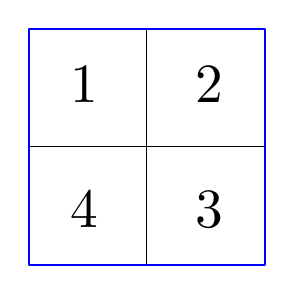
\begin{tikzpicture}[scale=.75, line join=round, line cap=round, >=stealth]
			\tikzset{every node/.style={thick,scale=2}}
			\def\R{2}  \def\r{.2} \def\d{1.5} 
			\path  (0,0)  coordinate (O) 
			(0:\R) coordinate (A)
			(90:\R) coordinate (B)
			(180:\R) coordinate (C)
			(-90:\R) coordinate (D)
			;
			\foreach \x in {A,B,C,D}{\draw (O)--(\x);}
			\draw[blue, thick] (-\R,-\R) rectangle (\R,\R);
			\draw (45:\d) node{$2$} (135:\d) node{$1$} (-135:\d) node{$4$} (-45:\d) node{$3$};
		\end{tikzpicture}
	\end{center}
	Có bao nhiêu cách để người thợ sơn có thể dùng bốn màu khác nhau để sơn tấm tường này sao cho mỗi ô vuông được tô một màu và những ô vuông cạnh nhau không có màu trùng nhau?
	\par\shortans[oly]{84}
	\loigiai{
		\begin{itemize}
			\item \textbf{Trường hợp 1:} Ô số 1 và ô số 3 cùng màu.\\
			Chọn màu cho ô số 1: có 4 cách.\\ 
			Chọn màu cho ô số 3: có 1 cách.\\
			Hai ô số 2 và 4 đều có cùng số cách chọn là 3.\\
			Số cách chọn màu trong trường hợp này là: $4\cdot 1\cdot 3\cdot 3=36$.
			\item \textbf{Trường hợp 2:} Ô số 1 và ô số 3 không cùng màu.\\
			Chọn màu cho ô số 1: có $4$ cách. \\
			Chọn màu cho ô số 3: có $3$ cách.\\
			Hai ô số 2 và 4 đều có cùng số cách chọn là 2.\\
			Số cách chọn màu trong trường hợp này là $4\cdot 3\cdot 2\cdot 2=48$.
		\end{itemize}
		Vậy số cách chọn màu thỏa mãn là $36+48=84$.
	}
\end{ex}

\begin{ex}%[0D8V1-5]%[Dự án đề cương 3 khối NH24-25-Dot 1-Thy Nguyen Vo Diem]
	Từ các chữ số $0$, $1$, $2$, $3$, $4$, $5$ có thể lập được bao nhiêu số tự nhiên gồm bốn chữ số phân biệt và chia hết cho $4$?
	\par\shortans[oly]{72}
	\loigiai{
		Gọi số tự nhiên cần tìm là $\overline{abcd}$.\\
		\textbf{Nhận xét:} Một số tự nhiên (gồm nhiều chữ số) chia hết cho 4 khi hai chữ số cuối của nó hình thành một số tư nhiên chia hết cho $4$.\\
		Theo đề, ta có $\overline{cd} \in  \{04,12,20,24,32,40,52\}$.\\
		\textbf{Trường hợp 1:} $\overline{c d} \in\{04,20,40\}$, có 3 cách chọn $\overline{c d}$.\\
		Chọn $a$: có 4 cách; chọn $b$: có $3$ cách.\\
		Vậy số các số thỏa mãn là $3 \cdot 4 \cdot 3=36$ (số).\\
		\textbf{Trường hợp 2:} $\overline{cd} \in\{12,24,32,52\}$, có $4$ cách chọn.\\
		Chọn $a$: có $3$ cách; chọn $b$: có $3$ cách. Số các số thỏa mãn là $4\cdot 3 \cdot 3=36$.\\
		Vậy số các số tự nhiên thỏa đề bài là $36+36=72$ (số).
	}
\end{ex}
\Closesolutionfile{ans}


\ind{PHẦN IV.} \inden{Tự luận.}\\
\setcounter{ex}{0}
\begin{ex}%[0D8H1-5]%[Dự án đề cương 3 khối NH24-25-Dot 1-Thy Nguyen Vo Diem]
	Có bao nhiêu số tự nhiên có ba chữ số, trong đó chữ số hàng trăm là chữ số chẵn, chữ số hàng đơn vị là chữ số lẻ?
	\loigiai{
		Ký hiệu số cần lập là $\overline{abc}$.\\
		Công việc gồm 3 bước là chọn chữ số hàng trăm, hàng chục và hàng đơn vị.\\
		Chữ số hàng trăm là số chẳn nên $a$ có $4$ cách chọn ($2$, $4$, $6$ hoặc $8$).\\
		Chữ số hàng đơn vị là số lẻ nên $c$ có $5$ cách chọn ($1$, $3$, $5$, $7$ hoặc $9$).\\
		Vị trí $b$ có $10$ cách chọn.\\
		Áp dụng quy tắc nhân, có $4 \cdot 5 \cdot 10 = 200$ số thỏa yêu cầu đề bài.
	}
\end{ex}
\begin{ex}%[0D8H1-3]%[Dự án đề cương 3 khối NH24-25-Dot 1-Thy Nguyen Vo Diem]
	An có thể đi từ nhà đến trường theo các con đường như hình dưới, trong đó có những con đường đi qua nhà sách.
	\begin{center}
		\begin{tikzpicture}[scale=1, font=\footnotesize, line join=round, line cap=round, >=stealth]
			\tkzDefPoints{0/0/A,3/0/B,6/0/C}
			\draw (C) arc [start angle=0, end angle=180, x radius=3, y radius=1];
			\draw (C) arc [start angle=0, end angle=-180, x radius=3, y radius=1];
			\draw (B) arc [start angle=0, end angle=180, x radius=3/2, y radius=1/2];
			\draw (B) arc [start angle=0, end angle=-180, x radius=3/2, y radius=1/2];
			\draw (C) arc [start angle=0, end angle=180, x radius=3/2, y radius=1/2];
			\draw (C) arc [start angle=0, end angle=-180, x radius=3/2, y radius=1/2];
			\draw (A) -- (B);
			\filldraw (A) circle (0.05) (B) circle (0.05) (C) circle (0.05);
			\draw (A) node[left]{Nhà An} (B) node[below=0.4]{Nhà sách} (C) node[right]{Trường};
		\end{tikzpicture}
	\end{center}
	\begin{enumerate}
		\item An có bao nhiêu cách đi từ nhà đến trường mà có đi qua nhà sách?
		\item An có bao nhiêu cách đi từ nhà đến trường?
	\end{enumerate}
	Lưu ý: Chỉ tính những con đường đi qua các điểm (nhà An, nhà sách, trường) không quá một lần.
	\loigiai{
		\begin{enumerate}
			\item Công việc gồm hai bước:\\
			\textit{Bước 1:} Đi từ nhà An đến nhà sách, có $3$ con đường.\\
			\textit{Bước 2:} Đi từ nhà sách đến trường, có $2$ con đường.\\
			Áp dụng quy tắc nhân, có $3 \cdot 2 = 6$ con đường để An đi từ nhà đến trường mà có đi qua nhà sách.
			\item Công việc có hai phương án thực hiện:\\
			\textit{Phương án 1:} An đi qua nhà sách, theo câu a, có $6$ con đường.\\
			\textit{Phương án 2:} An không đi qua nhà sách, có 2 con đường.\\
			Áp dụng quy tắc cộng, An có $6 + 2 = 8$ con đường đi từ nhà đến trường.
		\end{enumerate}
	}
\end{ex}	


\begin{ex}%[0D8N1-2]%[Dự án đề cương 3 khối NH24-25-Dot 1-Thy Nguyen Vo Diem]
	[\textit{Trích đề thi GKII - THPT Chuyên Lương Thế Vinh - Đồng Nai - Năm học 2024-2025}]
Một nhà hàng có thực đơn gồm $4$ món chính, $3$ món phụ, và $6$ loại đồ uống. Mỗi bữa trưa khách hàng chọn $1$ món chính, $1$ món phụ, và $1$ loại đồ uống. Hỏi có bao nhiêu cách chọn bữa trưa?
	\loigiai{
	\begin{itemize}
		\item Chọn món chính có $4$ cách chọn.
		\item Chọn món phụ có $3$ cách chọn.
		\item Chọn đồ uống có $6$ cách chọn.
	\end{itemize}
	Có tất cả $4\cdot 3\cdot 6=72$ cách chọn bữa trưa.
	}
\end{ex}

\begin{ex}%[0D8H1-2]%[Dự án đề cương 3 khối NH24-25-Dot 1-Thy Nguyen Vo Diem]
	Một thùng chứa $6$ quả dưa hấu, một thùng khác chứa $15$ quả thanh long. Từ hai thùng này,
	\begin{enumerate}
		\item có bao nhiêu cách chọn một quả dưa hấu hoặc một quả thanh long?
		\item có bao nhiêu cách chọn một quả dưa hấu và một quả thanh long?
	\end{enumerate}	
	\loigiai{
		\begin{enumerate}
			\item Công việc có hai phương án thực hiện:\\
			\textit{Phương án 1:} Chọn một quả dưa hấu, có $6$ cách chọn.\\
			\textit{Phương án 2:} Chọn một quả thanh long, có $15$ cách chọn.\\
			Áp dụng quy tắc cộng, có $6+15=21$ cách thực hiện.
			\item Công việc có hai công đoạn thực hiện:\\
			\textit{Công đoạn thứ nhất:} Chọn một quả dưa hấu, có $6$ cách chọn.\\
			\textit{Công đoạn thứ hai:} Chọn một quả thanh long, có $15$ cách chọn.\\
			Áp dụng quy tắc nhân, có $6 \cdot 15= 90$ cách thực hiện.
		\end{enumerate}
	}
\end{ex}

\begin{ex}%[0D8V1-1]%[Dự án đề cương 3 khối NH24-25-Dot 1-Thy Nguyen Vo Diem]
	Tính số giao điểm tối đa khi của $10$ đường thẳng phân biệt khi không có ba đường nào đồng quy và hai đường nào song song?
	\loigiai{
		Đường thẳng thứ nhất giao với 9 đường còn lại nên có 9 giao điểm.\\
		Đường thẳng thứ hai giao với 8 đường còn lại nên có thêm 8 giao điểm (đã tính giao điểm với đường thẳng thứ nhất ở trên).\\
		Đường thẳng thứ 9 giao với 1 đường còn lại nên có thêm 1 giao điểm.\\ 
		Vậy có $9+8+7+6+5+4+3+2+1=45$ giao điểm.
	}
\end{ex}

\begin{ex}%[0D8H1-1]%[Dự án đề cương 3 khối NH24-25-Dot 1-Thy Nguyen Vo Diem]
	Bạn Nam muốn mua một áo sơ mi cỡ $38$ hoặc cỡ $39$. Áo cỡ $38$ có $4$ màu khác nhau, áo cỡ $39$ có $6$ màu khác nhau. Hỏi bạn Nam có bao nhiêu sự lựa chọn để mua một cái áo sơ mi?
	\loigiai{
		Việc mua một áo sơ mi có $2$ phương án thực hiện:\\
		Chọn một áo sơ mi cỡ $38$ có $4$ cách khác nhau.\\
		Chọn một áo sơ mi cỡ $39$ có $6$ cách khác nhau.\\
		Số cách chọn để bạn Nam mua một áo sơ mi là $4+6=10$ cách.
	}
\end{ex}
%%%==============ex_55==============%%%
\begin{ex}%[0D8H1-1]
	Giả sử từ tỉnh $A$ đến tỉnh $B$ có thể đi bằng các phương tiện: ô tô, tàu hỏa, tàu thủy hoặc máy bay. Mỗi ngày có $8$ chuyến ô tô, $4$ chuyến tàu hỏa, $2$ chuyến tàu thủy và $2$ chuyến máy bay. Hỏi có bao nhiêu cách đi từ tỉnh $A$ đến tỉnh $B$ bằng một trong các phương tiện trên?
	\loigiai{
		Việc di chuyển từ tỉnh $A$ đến tỉnh $B$ có bốn phương án thực hiện:\\
		Di chuyển bằng ô tô, có 8 cách chọn chuyến.\\
		Di chuyển bằng tàu hỏa, có 4 cách chọn chuyến.\\
		Di chuyển bằng tàu thủy, có 2 cách chọn chuyến.\\
		Di chuyển bằng máy bay, có 2 cách chọn chuyến.\\
		Áp dụng quy tắc cộng, ta có số cách chọn để di chuyển từ $A$ đến $B$ là $8+4+2+2=16$ cách.
	}
\end{ex}

\begin{ex}%[0D8H1-1]%[Dự án đề cương 3 khối NH24-25-Dot 1-Thy Nguyen Vo Diem]
	Trong một trường THPT, khối $10$ có $240$ học sinh nam và $315$ học sinh nữ. Nhà trường cần chọn một học sinh ở khối $10$ đi dự khai mạc hội thi Robocon dành cho học sinh thành phố. Hỏi nhà trường có bao nhiêu cách chọn?
	\loigiai{
		Việc chọn một học sinh khối $10$ đi dự khai mạc hội thi có hai phương án thực hiện:\\
		Chọn một học sinh nam có $240$ cách.\\
		Chọn một học sinh nữ có $315$ cách.\\
		Theo quy tắc cộng, số cách chọn một học sinh khối $10$ đi dự khai mạc hội thi là 
		$240+315=555$ cách.
	}
\end{ex}

\begin{ex}%[0D8H1-1]%[Dự án đề cương 3 khối NH24-25-Dot 1-Thy Nguyen Vo Diem]
	Một hộp chứa năm quả cầu trắng được đánh số từ $1$ đến $5$ và bốn quả cầu đen được đánh số từ $6$ đến $9$. Có bao nhiêu cách chọn một quả cầu từ hộp?
	\loigiai{
		Việc chọn một quả cầu có hai phương án thực hiện:\\
		Chọn một quả cầu trắng có $5$ cách.\\
		Chọn một quả cầu đen có $4$ cách.\\
		Theo quy tắc cộng, số cách chọn một quả cầu từ hộp là: $5+4=9$ cách.
	}
\end{ex}

\begin{ex}%[0D8V1-2]%[Dự án đề cương 3 khối NH24-25-Dot 1-Thy Nguyen Vo Diem]
	Biển số xe máy của tỉnh $A$ (nếu không kể mã số tỉnh) có $6$ kí tự, trong đó kí tự ở vị trí đầu tiên là một chữ cái (trong bảng 26 cái tiếng Anh), kí tự ở vị trí thứ hai là một chữ số thuộc tập $\{1; 2; \ldots; 9\}$ mỗi kí tự ở bốn vị trí tiếp theo là một chữ số thuộc tập $\{0; 1; 2; \ldots; 9\}$. Hỏi nếu chỉ dùng một mã số tỉnh thì tỉnh $A$ có thể làm được nhiều nhất bao nhiêu biển số xe máy khác nhau?
	\loigiai{
		Giả sử biển số xe là $\overline{abcdef}$.\\ 
		Có 26 cách chọn $a$;\\ 
		Có 9 cách chọn $b$;\\ 
		Có 10 cách chọn $c$;\\ 
		Có 10 cách chọn $d$;\\ 
		Có 10 cách chọn $e$;\\ 
		Có 10 cách chọn $f$.\\ 
		Vậy có $26\cdot 9\cdot 10\cdot 10\cdot 10\cdot 10=2340000$ biển số xe.
	}
\end{ex}